% This text is proprietary.
% It's a part of presentation made by myself.
% It may not used commercial.
% The noncommercial use such as private and study is free
% Sep. 2005 
% Author: Sascha Frank 
% University Freiburg 
% www.informatik.uni-freiburg.de/~frank/


\documentclass{beamer}
\setbeamertemplate{frametitle}
 	{\begin{centering}\smallskip
    \insertframetitle\par
    \smallskip\end{centering}}
\setbeamertemplate{itemize item}{$\bullet$}
\setbeamertemplate{navigation symbols}{}
\setbeamertemplate{footline}[text line]{%
    \hfill\strut{%
	\scriptsize\sf\color{black!60}%
	\quad\insertframenumber
	}%
    \hfill
    }    
    % Define some colors:
    \definecolor{DarkFern}{HTML}{407428}
    \definecolor{DarkCharcoal}{HTML}{4D4944}
    \colorlet{Fern}{DarkFern!85!white}
    \colorlet{Charcoal}{DarkCharcoal!85!white}
    \colorlet{LightCharcoal}{Charcoal!50!white}
    \colorlet{AlertColor}{orange!80!black}
    \colorlet{DarkRed}{red!70!black}
    \colorlet{DarkBlue}{blue!70!black}
    \colorlet{DarkGreen}{green!70!black}
     
    % Use the colors:
    \setbeamercolor{title}{fg=Fern}
    \setbeamercolor{frametitle}{fg=Fern}
    \setbeamercolor{normal text}{fg=Charcoal}
    \setbeamercolor{block title}{fg=black,bg=Fern!25!white}
    \setbeamercolor{block body}{fg=black,bg=Fern!25!white}
    \setbeamercolor{alerted text}{fg=AlertColor}
    \setbeamercolor{itemize item}{fg=Charcoal}

  \usepackage[T1]{fontenc}
  \usepackage[utf8]{inputenc}
  \usepackage{lmodern}
  \usepackage[french]{babel}
\begin{document}
\title{Compter les points sur une courbe elliptique}   
\author{Jeremie Coulaud} 
\date{\today} 

\frame{\titlepage} 

\frame{\frametitle{Table of contents}\tableofcontents} 


\section{Introduction} 
\frame{\frametitle{Introduction} 
blabla
}

\section{Algorithme naïf}
\frame{\frametitle{Algorithme naïf}
$$ y^2 = x^3 +ax+b = f(x) $$
\begin{itemize}
\item  $\genfrac(){}{0}{f(x)}{p} = -1$, $f(x)$ n'est pas un carré modulo $p$, on ne trouve aucun point appartenant à la courbe.
\item $\genfrac(){}{0}{f(x)}{p} = 0$, $f(x)$ est divisible par $p$, on trouve $1$ point sur la courbe.
\item $\genfrac(){}{0}{f(x)}{p} = 1$, $f(x)$ est un carré modulo $p$, on trouve $2$ points sur la courbe.
\end{itemize}
}

\begin{frame}
\frametitle{}
\begin{equation*}
\#E(\mathbb{F}_p) = 1 + p +\sum_{x \in \mathbb{F}_p}\genfrac(){}{0}{f(x)}{p}
\end{equation*}
Complexité en la taille de $p$
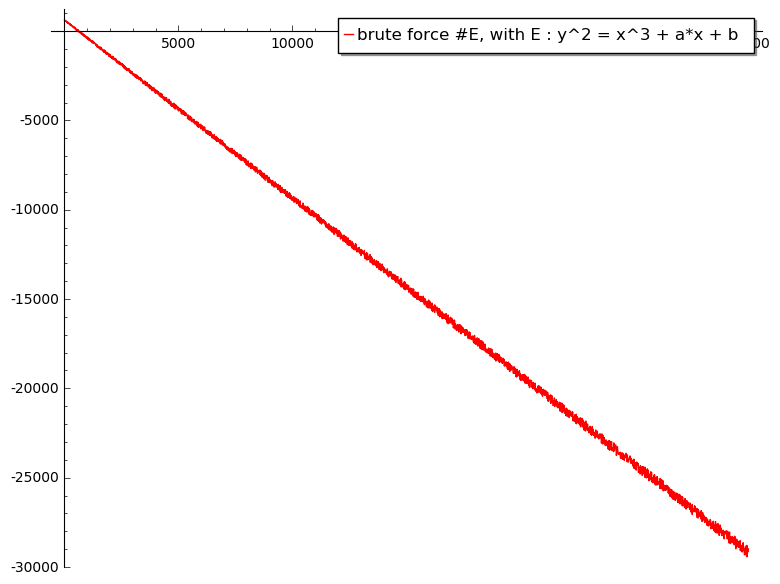
\includegraphics[scale=0.4]{../pictures/brute_force_cputime.png} 
\end{frame}

\section{Algorithme de Schoof}
\begin{frame}
\frametitle{Algorithme de Schoof}

\begin{block}{Théorème Hasse-Weil}
$\#E(\mathbb{F}_p) = p + 1 - t$ avec $|t| \leq 2 \sqrt{p}$ trace de l'endomorphisme de Frobenius de $E$.
\end{block}
Pour trouver l'ordre de $E(\mathbb{F}_p)$ il faut trouver $t$
\newline
Idée de Schoof : trouver $t \pmod l$, avec $l$ petit premier et utiliser les restes chinois pour trouver $t$
\end{frame}

\subsection{Frobenius}
\begin{frame}
\frametitle{Frobenius}
Soit $E$ une courbe elliptique défini sur $\mathbb{F}_p$, l'endomorphisme de Frobenius est défini par 

$\begin{array}{ccccc}
\phi_p & : & E(\mathbb{F}_p) & \to & E(\mathbb{F}_p) \\
 & & (x,y) & \mapsto & (x^p, y^p) \\
\end{array}$

On lui associe son polynôme caractéristique :
\begin{equation*}
\phi_p^2 - t \phi_p + p = 0
\end{equation*}
\end{frame}

\end{document}

